\chapter{全景漫游行业的市场现状}

\section{全景漫游技术总览}

全景漫游技术按载体分类可分为:
\begin{enumerate}
\item{\emph{场景捕获硬件技术:}视频捕获设备及其保障设备,用以采集全景漫游的视频、图片、音频等素材。}
\item{\emph{场景呈现硬件技术:}主要包括 VR 眼镜、VR 互动手柄、VR 主机等。}
\item{\emph{场景处理技术:}场景规划设计、场景素材的保存与传输以及相应程序开发等。}
\item{\emph{场景还原与增强技术:}将场景素材与功能模块有机地整合,提供给用户身临其境般的全景漫游体验。}
\end{enumerate}

\subsection{场景呈现硬件技术}
相对而言,硬件技术相比于后两者进入门槛更高。目前市场上三大 VR 硬件厂商 OculusRift、HTCVive 和 PlayStationVR 几乎垄断了高端 VR 播放设备市场。之后加入 VR 市场的企业(如暴风、大朋、3Glasses、蚁视等)几乎都放低了姿态,推出了价格低廉但基本满足播放功能的入门级 VR 眼镜作为卖点。但随着 Google Cardboard 的推出,这款几乎没有成本可言的开源“硬件”迅速占领了低端 VR 硬件行业相当客观的市场份额。

\subsection{场景捕获硬件技术}
场景捕获技术的难点在于实时捕获,合成全景照片是一般手机都拥有的功能,大致原理就是捕获数张连续且相近的照片并通过算法进行合成球形场景。但实时场景捕获硬件的成本因其同步的特性更为高昂,目前市面上已有的厂商例如 Google JUMP、NOKIA OZO 等均是将现有平面镜头进行堆叠排布并通过后期处理合成虚拟场景,且这种方式因需要较多的镜头来堆砌同时刻的画面所以硬件成本非常高。目前市面上尚只有堆叠摄像头这一种方式进行全景场景捕获,而光场摄影等技术仍处在技术攻关阶段,相信不远的将来有可能出现消费级的场景捕获硬件。

\subsection{场景处理技术}
场景处理是目前全景漫游软件领域需要重点攻克的最大难关,但市面上各企业已基本做到自给自足的技术支持。全景漫游所依赖的基础是图像信号的捕获、加工与储存,而这些方面已有较多成功经验。目前 Web 端视频播放协议有以下两种:Real Time Messaging Protocol(实时消息传输协议,简称 RTMP)和 HTTP Live Streaming(HTTP 渐进下载,简称 HLS)。这两者是孑然不同的两种协议,而且 iPhone 等手机由于不自带支持 Flash 播放,一般考虑全端支持的流媒体播放会选用 HLS 作为传输协议,即对视频做切片,边播放边加载下一时段的切片。

\subsection{场景还原与增强技术}
场景还原与增强是与用户直接相连的部分,可以说前面的技术都是起为其保驾护航的功能。其中场景还原部分为计算机图形学的范畴,例如图像在空间上的曲率计算等,主要涉及到的技术有 OpenGL/WebGL 等,用于将二维图像还原成球状的场景。而场景增强技术则是本文所讨论的重点,其又分前处理和后处理两种,但因场景搭建的过程比较复杂,所以两种处理模式界限并不是特别清晰。

\paragraph{场景前处理代表:Unity3D}

Unity3D 是由 Unity Technologies 开发的一个让玩家轻松创建诸如三维视频游戏、建筑可视化、实时三维动画等类型互动内容的多平台的综合型游戏开发工具,是一个全面整合的专业游戏引擎。\endnote{http://t.cn/RJDzA1F}

\paragraph{场景后处理代表:Krpano}
Krpano 是一个小巧灵活的用来呈现各种全景图像和交互式的虚拟之旅的高性能全景查看器。可作为 Flash 和 HTML5 应用程序在 Web 上使用。并附有利用拖拽全景生成场景的 Krpano Tools 以供开发者快速生成用以展示的全景场景。本文将应用其进行部分设计案例的制作与演示。

\paragraph{场景后处理代表:Aframe}
Aframe 是一个用 Web 技术构建 VR 体验的框架。使用 HTML 语言及实体组件来构建场景,可应用于 web/mobile 和其他多种设备端。本文将应用其进行部分设计案例的制作与演示。

\section{全景漫游市场前景}

2016 年,随着三大 VR 设备开始出售,未来 2-3 年 VR 设备普及率将快速提升。到达 2020 年,虚拟现实生态圈将初步形成,内容、服务等盈利模式逐步成熟,全球 VR 市场规模将达到 404 亿美元,VR 游戏市场规模将达到 149.5 亿美元。\endnote{http://vreyes.baijia.baidu.com/article/595977}

虚拟现实(VR/AR)产业市场具有良好前景,2015 年中 国虚拟现实行业市场规模为 15.4 亿元人民币。融资方面,国内 VR/AR 领域投资活跃度从 2015 年开始显著提升,2015 年第四季度和 2016 年第一季度的融资额均接近 10 亿元。其中显示设备融资占据首要地位,2015 年融资案例数量占比 30\%,融资额占比 69\%;内容制作的融资案例数量虽然占比 22\%,但融资额仅占比 6\%\endnote{http://www.elecfans.com/vr/444138.html}。可见 VR 及全景漫游方向的内容制作生产领域仍处于起步阶段,与硬件厂商等差距较大,但同时其中也孕育了巨大的商机。

VR 内容开发受市场认可,线下体验馆增长迅速。由于中国 VR 市场主流设备仍以移动端 VR 眼镜为主,VR 视频内容的开发数量要远多于 VR 游戏内容。VR 平台上已有约 2700 款视频和 800 款游戏。预计 2020 年中国 VR 设备出货量 820 万台,用户量超过 2500 万人,见图\ref{fig:market}。

\begin{figure}[h]
\centering
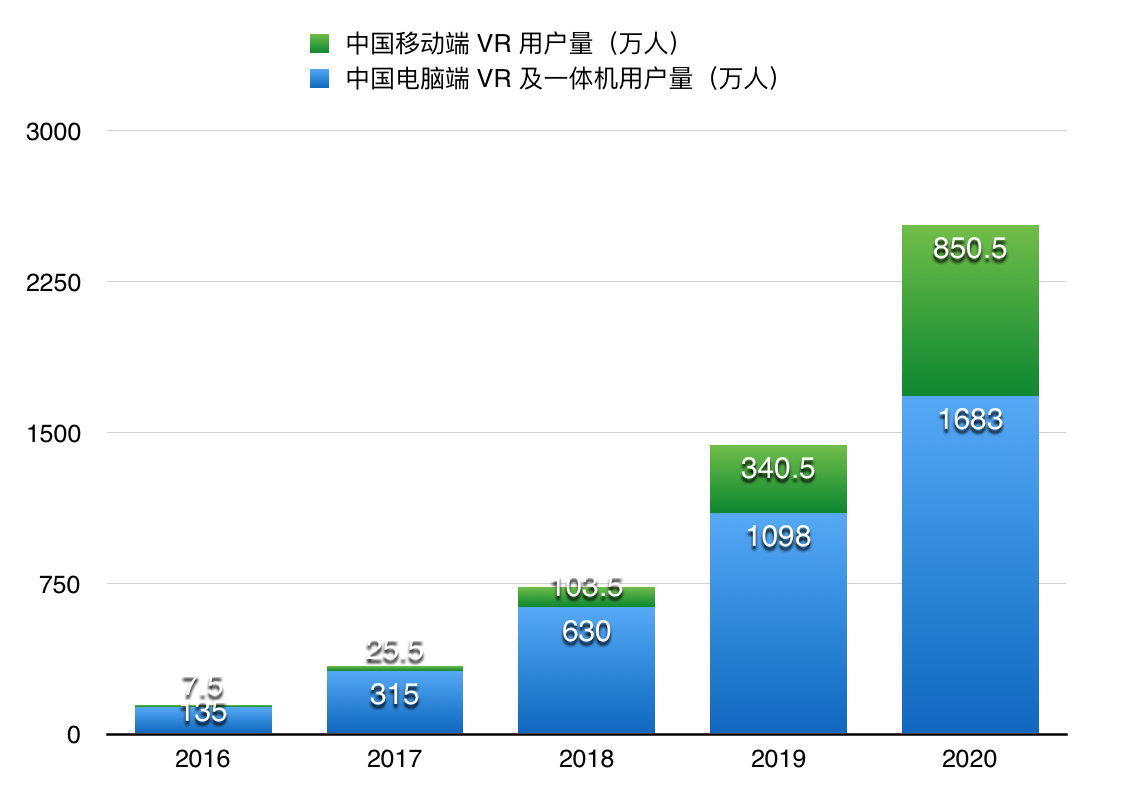
\includegraphics[width=.4\textwidth]{market}
\caption{2016-2020 年中国 VR 用户规模}
\label{fig:market}
\end{figure}

\section{全景漫游产业类别}
全景漫游产业按出发点可大体分为两类:
\begin{itemize}
	\item 以视频、游戏为主的虚拟内容提供商/平台商
	\item 涉及电商、教育、医疗、建筑等传统行业的行业融合应用服务商
\end{itemize}

短期而言,市场上比较活跃的是虚拟内容提供商,但长远而言,ToB 模式更利于产生更为健壮的全景漫游服务体系,对于高质内容的生产、分发和变现的模式也偏向于有传统大规模企业的行业服务商。

\section{全景漫游现有 APP 分析}
\subsection{Ascape}

Ascape 这款美国公司开发的应用于 2017 年发布,主攻虚拟旅游市场。你能够通过 360° 无缝的全景视频身临其境般地切身体验视频中呈现的著名景点或人文古迹,探索只有历经千难万险才能体会的绮丽风光。伴随着你的移动,场景中镜头也会随之改变整个画面的位置和显示的角度,见图\ref{fig:ascape1}。

\begin{figure}[htp]
\centering
\fbox{
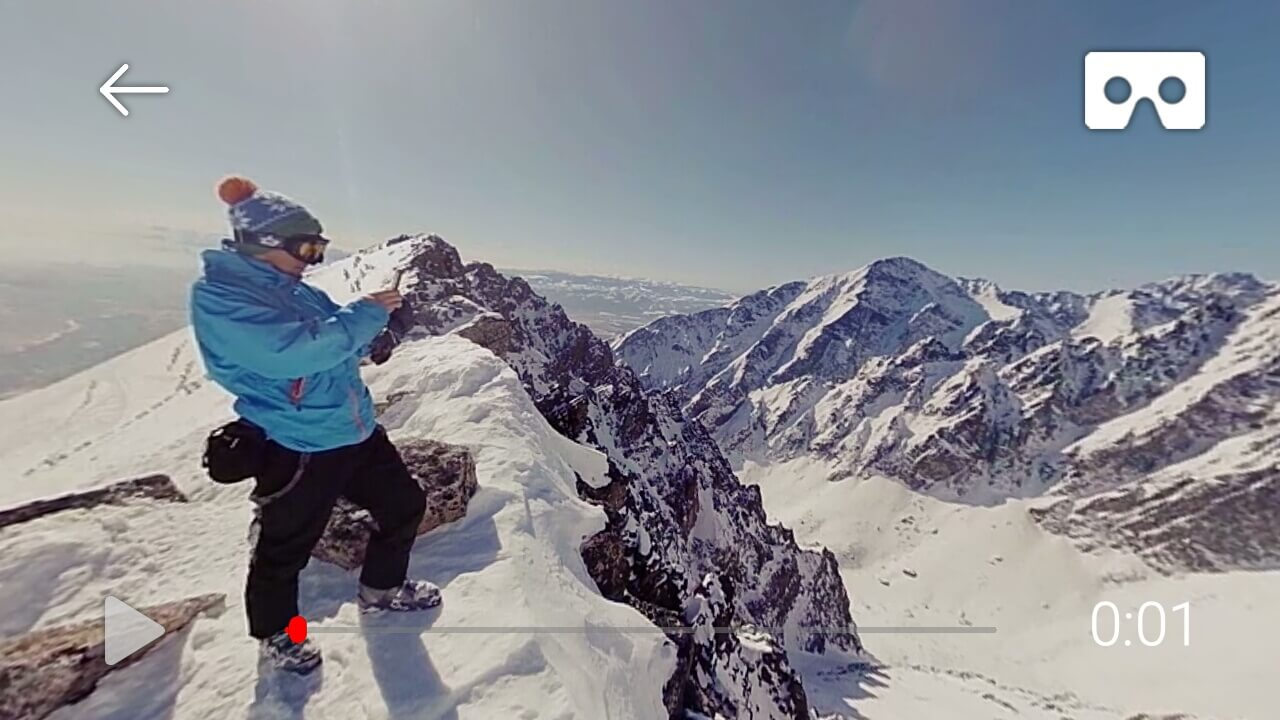
\includegraphics[width=.7\textwidth]{ascape2}
}
\caption{简洁的全景视频播放}
\label{fig:ascape1}
\end{figure}

同时,这款应用在移动应用传统界面上也继承了欧美一向以来的简约风格:“探索”页面采用卡片设计模式直观展示了新奇的场景;“发现”页面通过地图和名单两种模式展示了全球各地的场景选项;“我的旅行”也通过卡片模式展示了已下载的全景场景,见图\ref{fig:ascape2}。

\begin{figure}[htp]
\centering
\fbox{
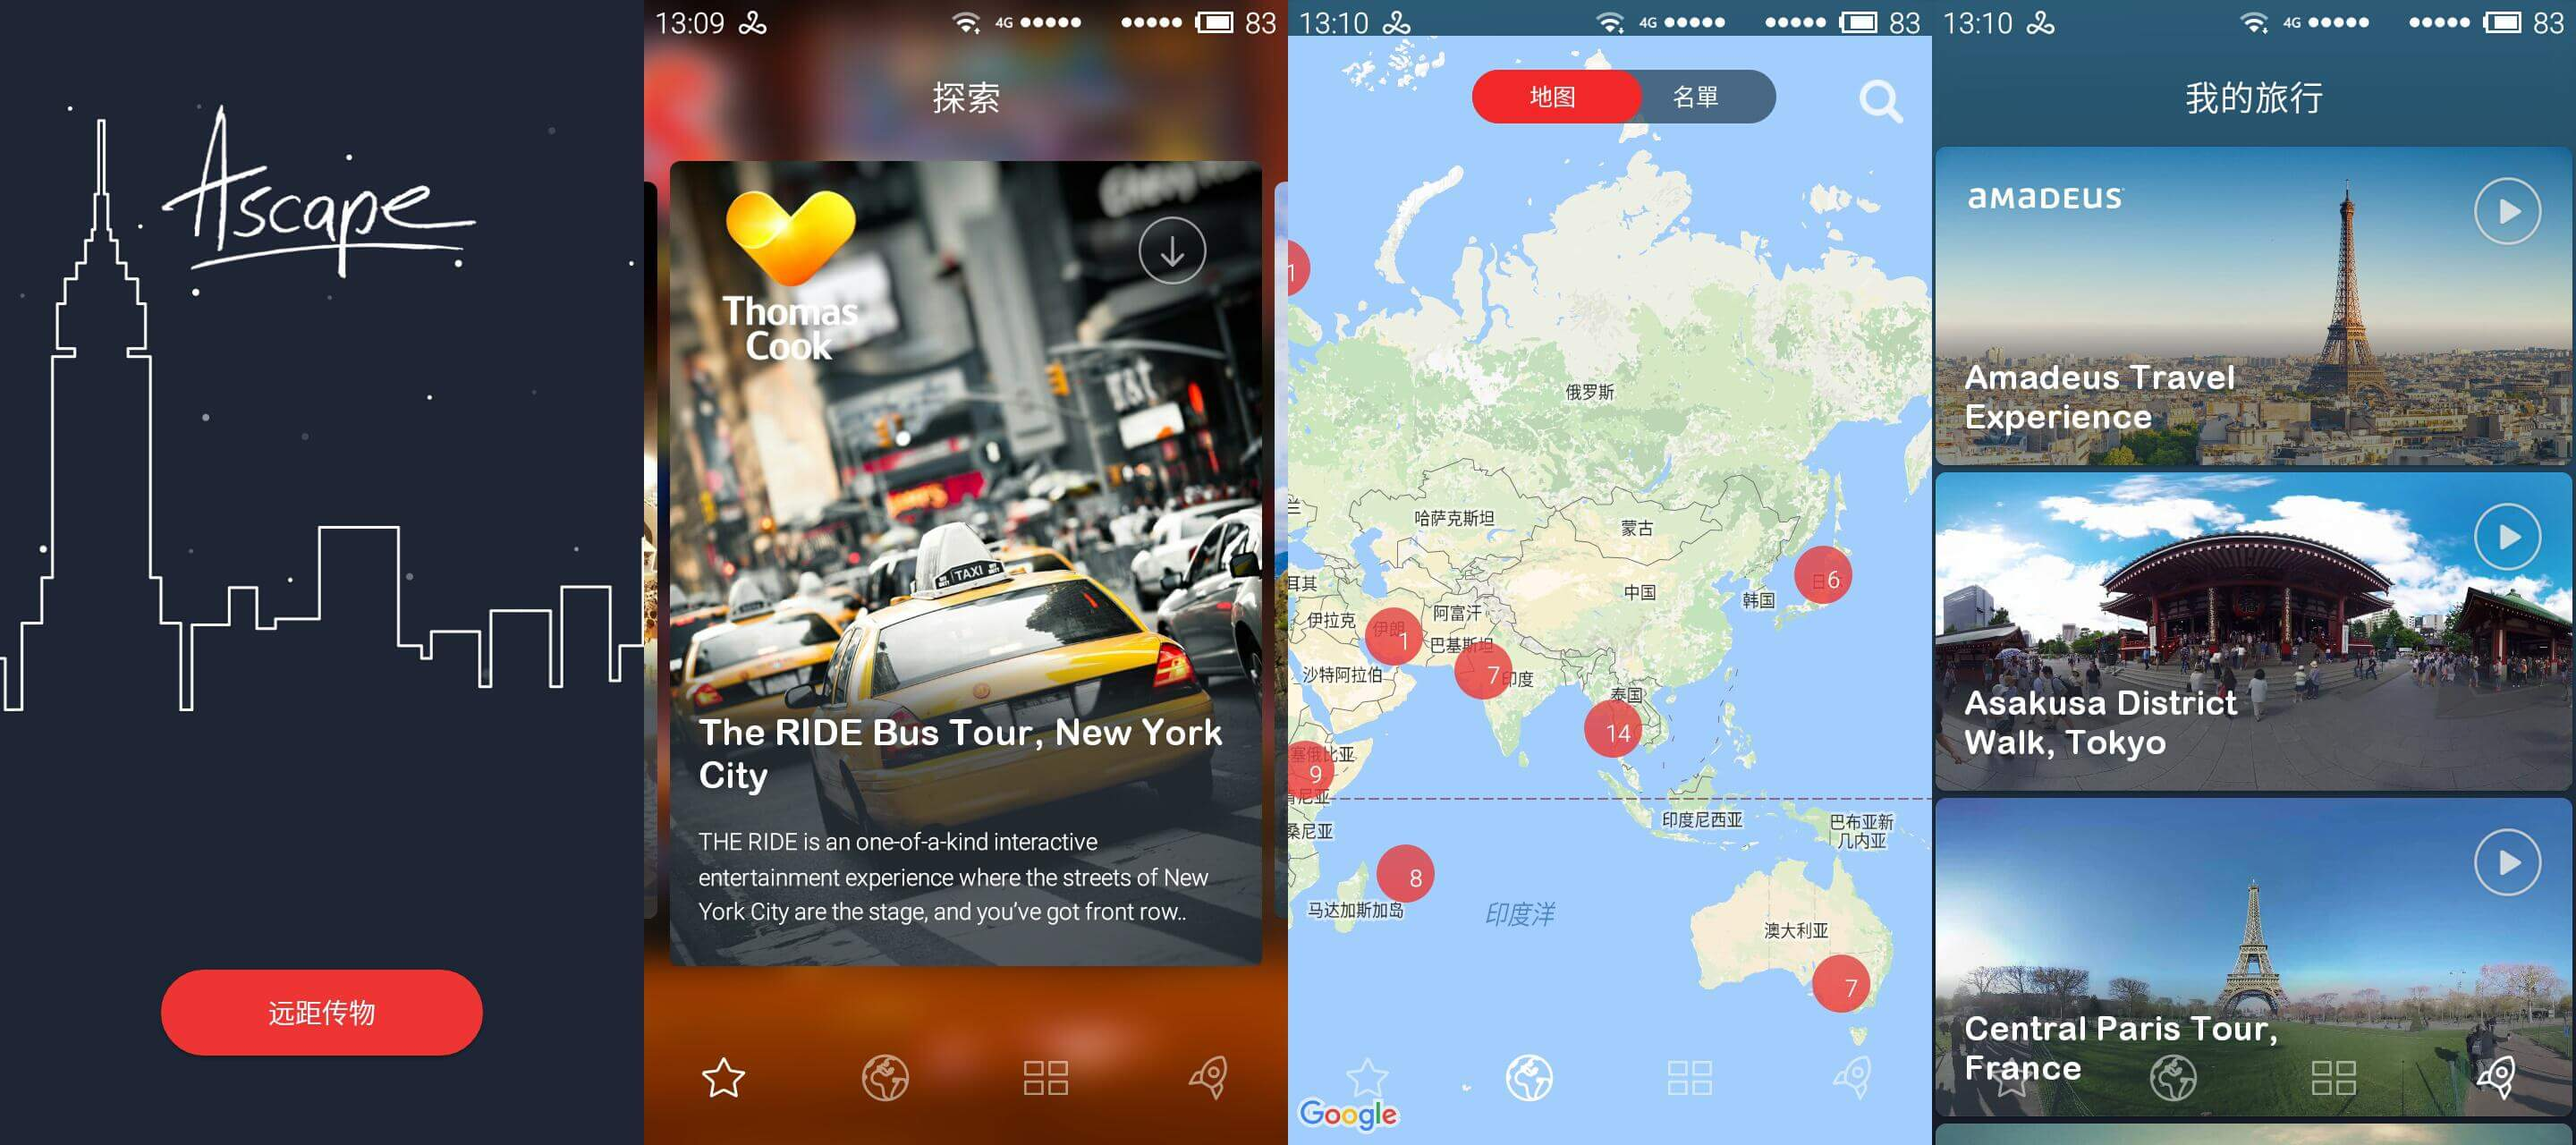
\includegraphics[width=.7\textwidth]{ascape1}
}
\caption{简洁的全景视频播放}
\label{fig:ascape2}
\end{figure}

\subsection{Fulldive}

Fulldive 这款美国公司开发的应用于 2016 年发布,是一个智能手机与虚拟场景连接的平台,进入应用后即进入了一个全景漫游的世界。场景内包含常用的网络视频、本地视频/图片、VR 相机、VR 浏览器等应用,同时支持从其内部市场下载更多基于其开发的虚拟现实应用,见图\ref{fig:fulldive1}。

\begin{figure}[htp]
\centering
\fbox{
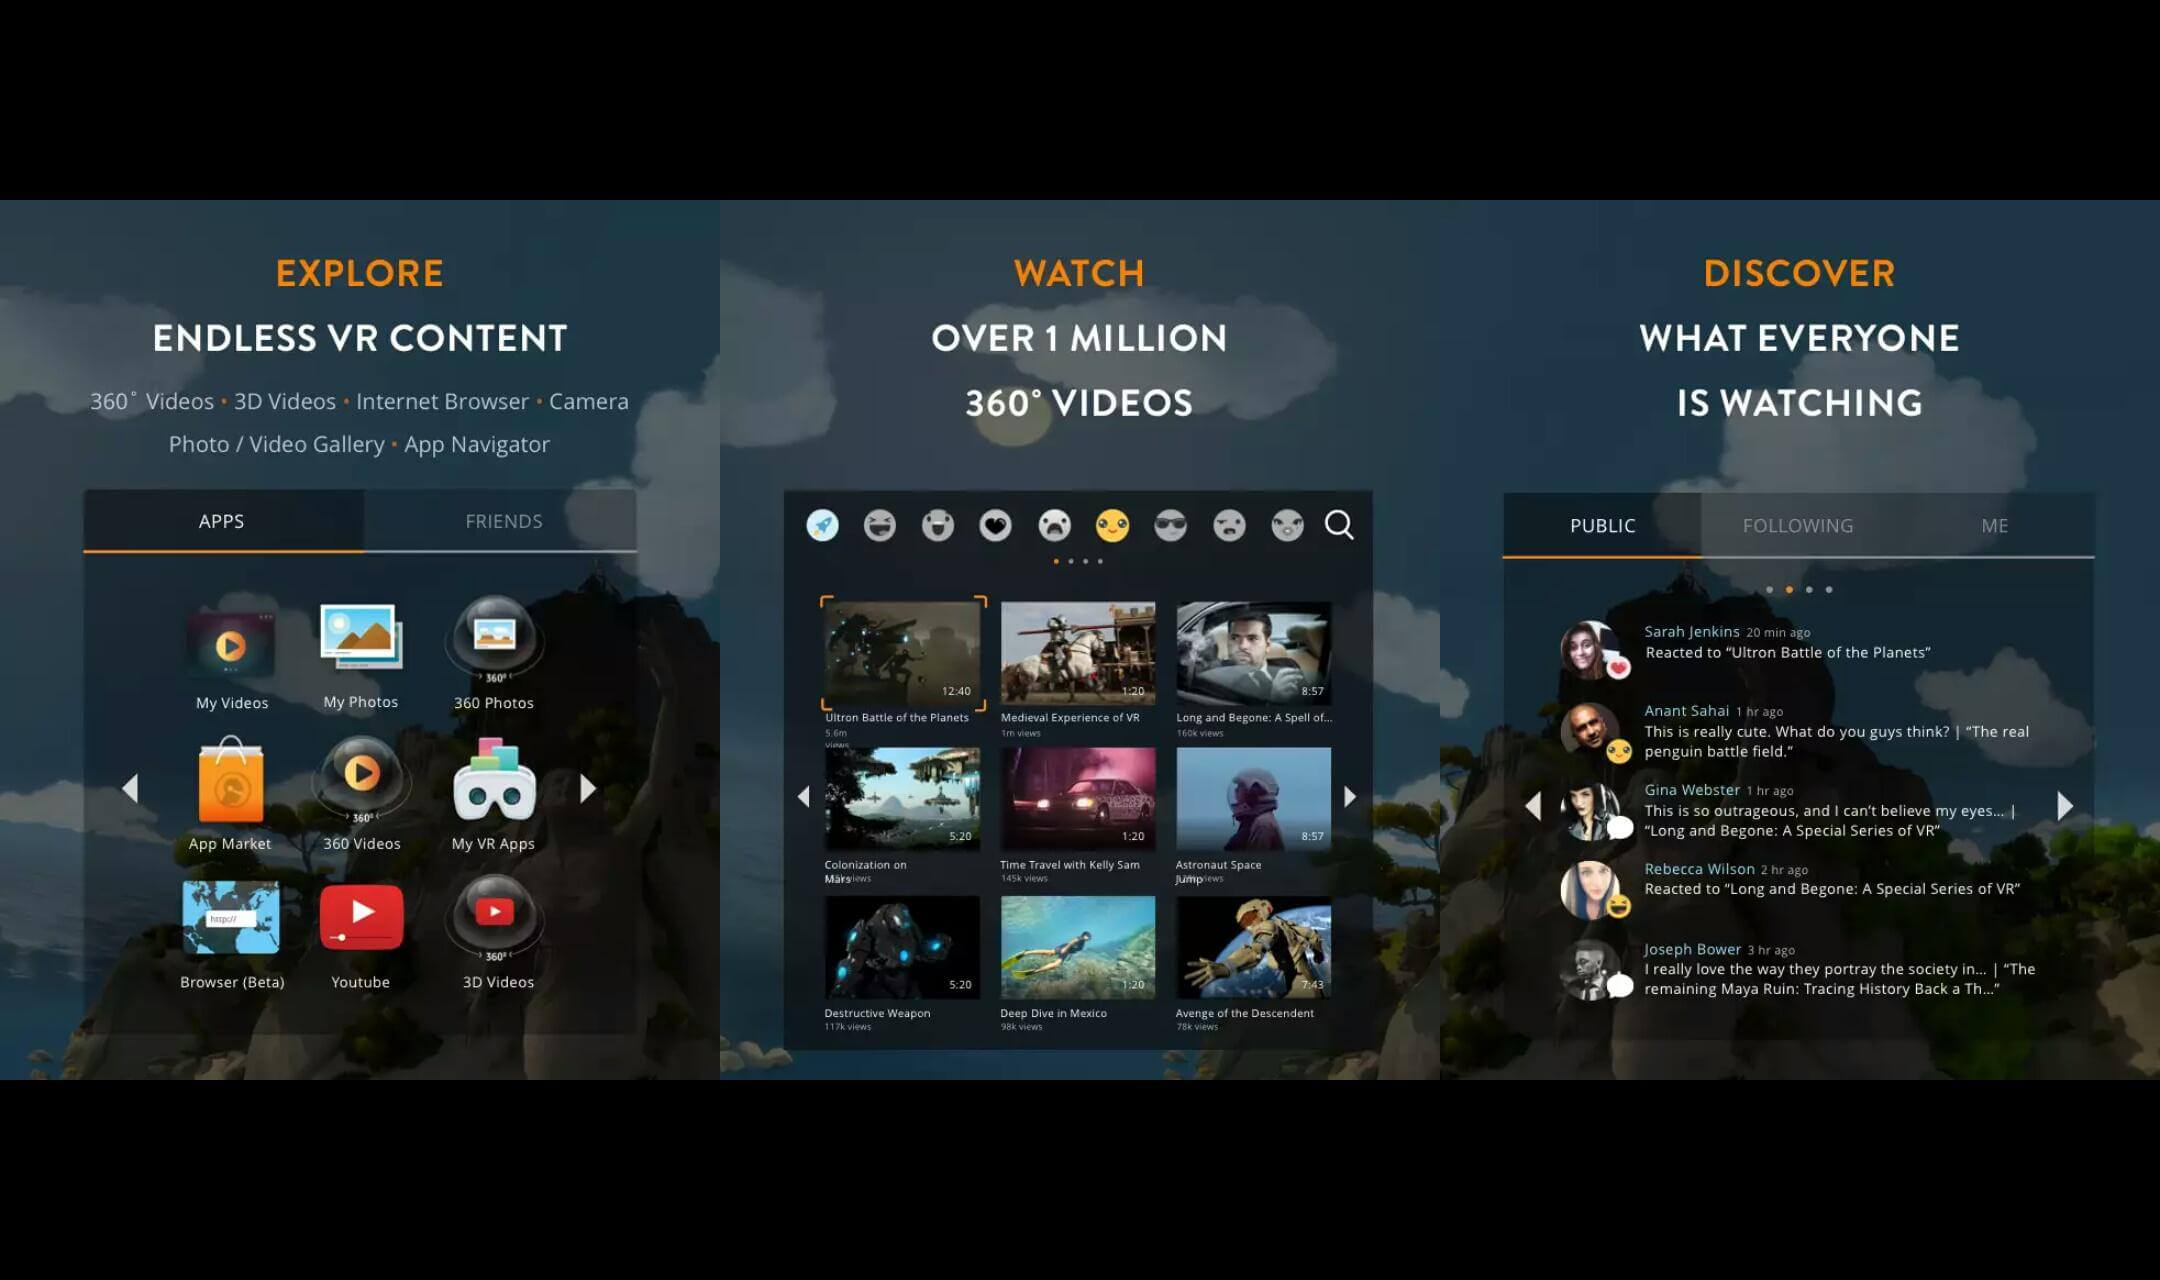
\includegraphics[width=.7\textwidth]{fulldive1}
}
\caption{Fulldive 内置的应用列表}
\label{fig:fulldive1}
\end{figure}

与 Ascape 不同之处在于 Fulldive 的操控完全是在虚拟全景中,所以在播放视频及操作选项时 Fulldive 有一些针对配戴虚拟现实眼镜者所特别提供的操作方式,见图\ref{fig:fulldive2}。例如,将视线聚焦在某个按钮上超过 3 秒后即视为按下了该按钮。这种交互形式借鉴了鼠标的双击或是触屏的长按这两种操作,同时兼顾到视线对齐对人操作的便捷性和可操作性,见图\ref{fig:fulldive3}。

\begin{figure}[htp]
\centering
\fbox{
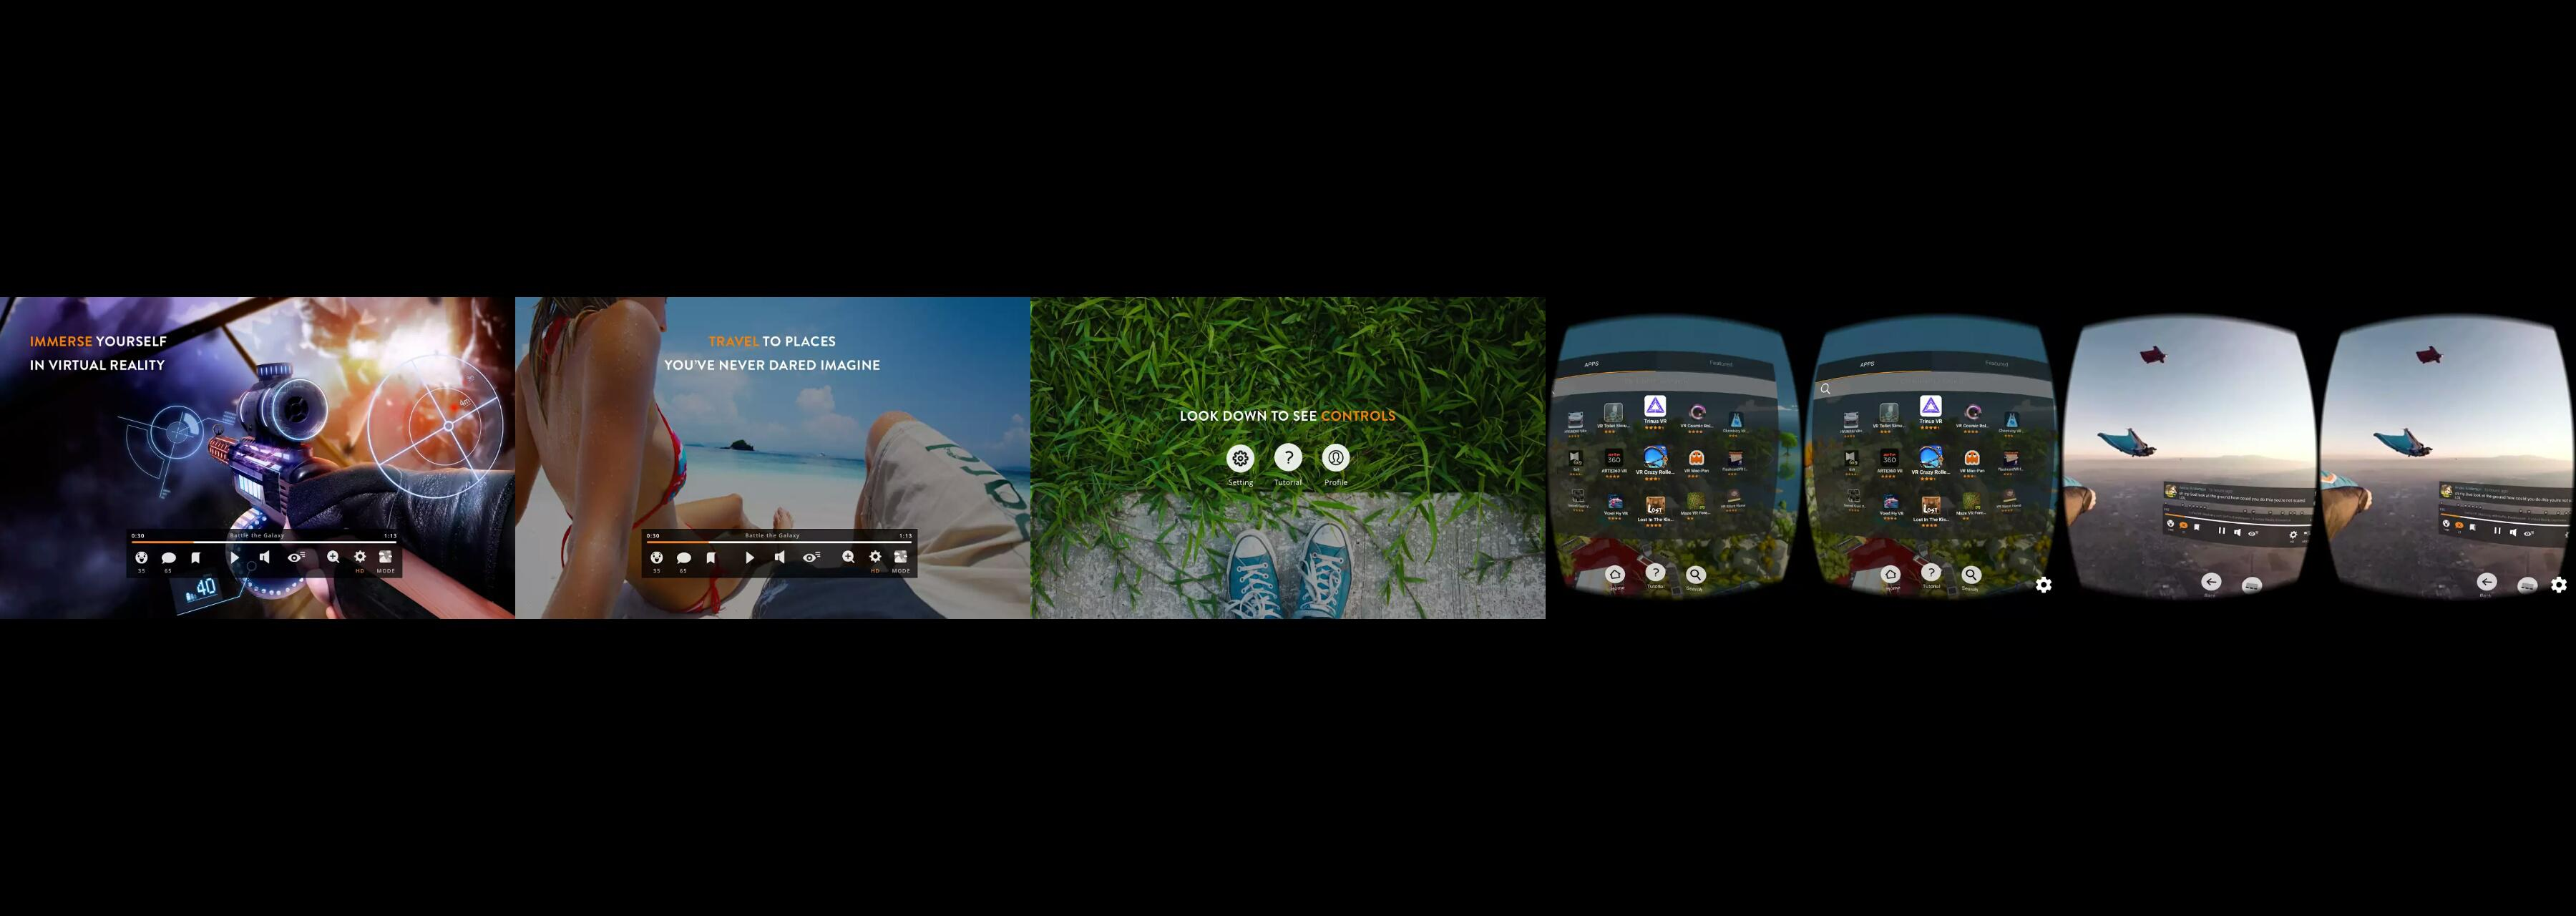
\includegraphics[width=.6\textwidth]{fulldive2}
}
\caption{Fulldive 特有操作形式}
\label{fig:fulldive2}
\end{figure}

\begin{figure}[htp]
\centering
\fbox{
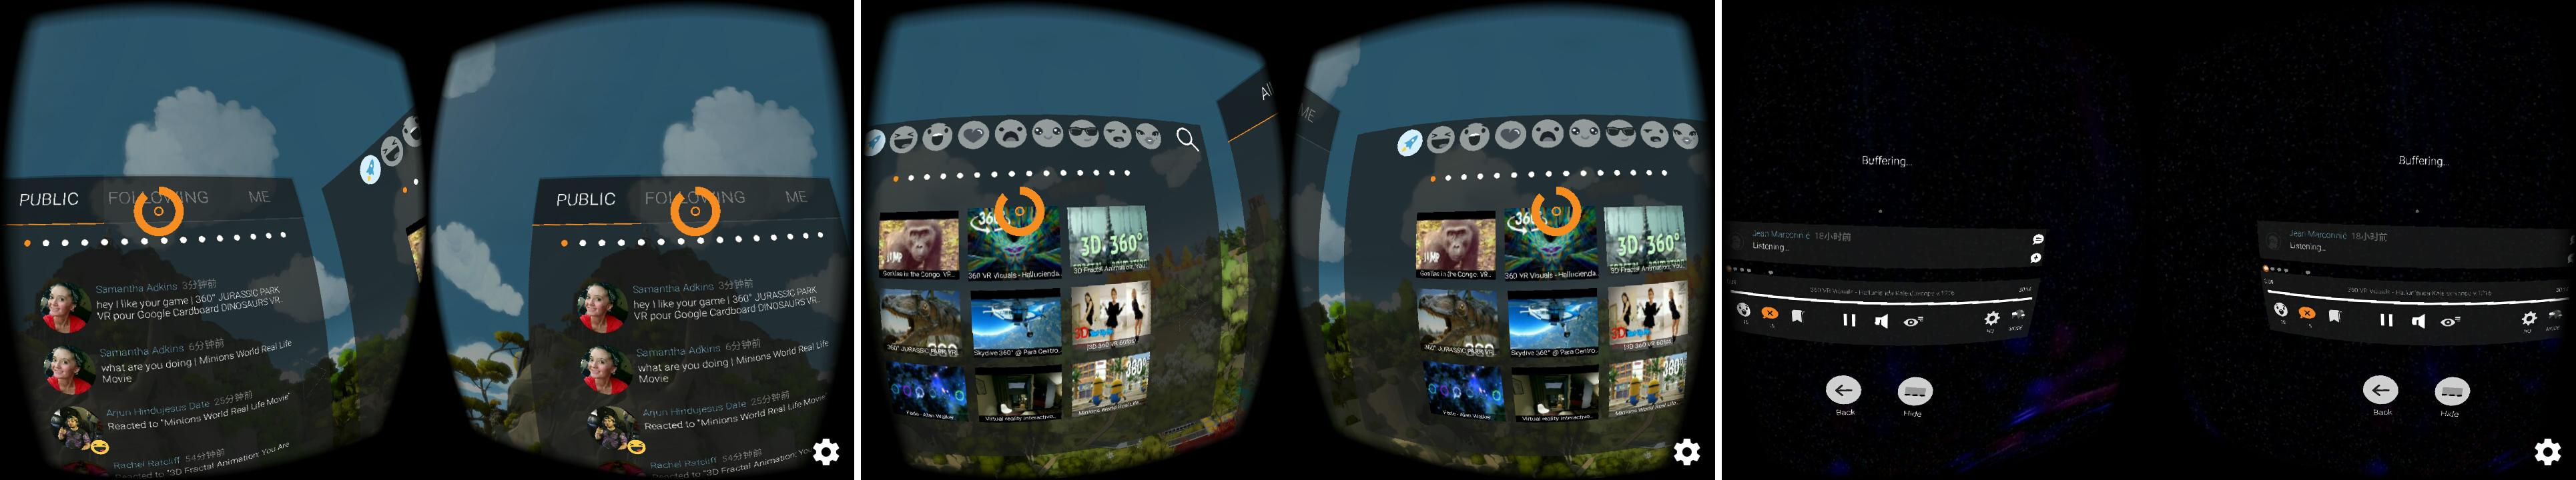
\includegraphics[width=.6\textwidth]{fulldive3}
}
\caption{Fulldive 视线停留模拟点击}
\label{fig:fulldive3}
\end{figure}

当然,这种模拟点击的操作只适用于”确认/取消“这种布尔判断的操作,用户需要输入大段的文字时则需有更高效的方式。Fulldive 结合了已日益成熟的语音识别技术,图\ref{fig:fulldive4}为实际操作 Fulldive 搜索功能并口述”中国地质大学“后的操作截屏。

\begin{figure}[htp]
\centering
\fbox{
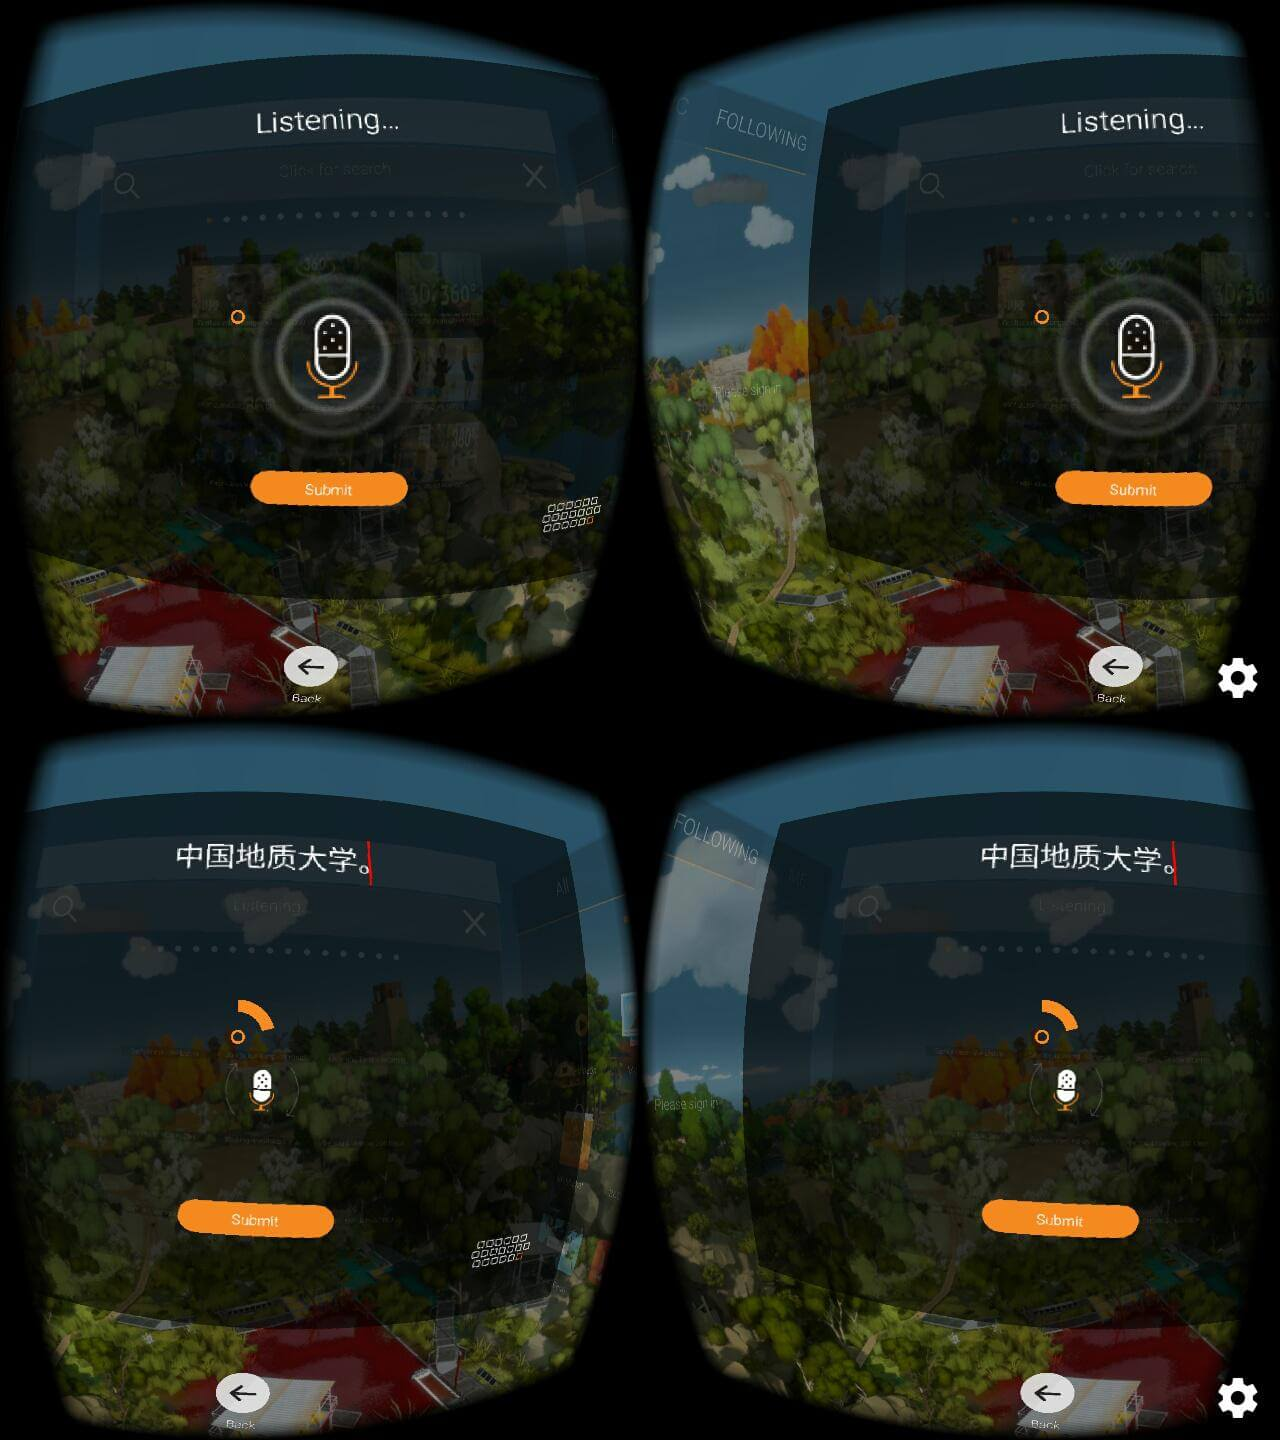
\includegraphics[width=.5\textwidth]{fulldive4}
}
\caption{Fulldive 语音识别}
\label{fig:fulldive4}
\end{figure}

\subsection{VR X-Racer}

VR X-Racer 是一款越南公司于 2016 年开发的简单的 VR 操控类飞行游戏,其操作方式为晃动设备(如 VR 眼镜或手机)来控制屏幕上的飞机躲避障碍物,见图\ref{fig:x-racer}。这是全景漫游技术在游戏上最直接的体现:几乎没有多余的操作,在游戏中飞机撞到障碍物坠毁后无操作若干秒即自动重新游戏。但其最大的缺陷是无法长时间使用,不断晃动的全景屏幕容易使人产生眩晕、恶心等不良反应。
全景漫游与 3D 影片的体验是完全不同的,全景漫游将用户完全包裹在视频所构建的封闭环境中,而 3D 眼镜只是对屏幕这种有限区域进行了折射。两者的区别在于 3D 影片由于有周围环境作为铺垫不易使人完全沉浸其中,全景漫游则是在很短的时间内(20-30 秒)就使人沉浸在虚拟世界中,直至摘掉全景设备重新适应周围环境。

\begin{figure}[htp]
\centering
\fbox{
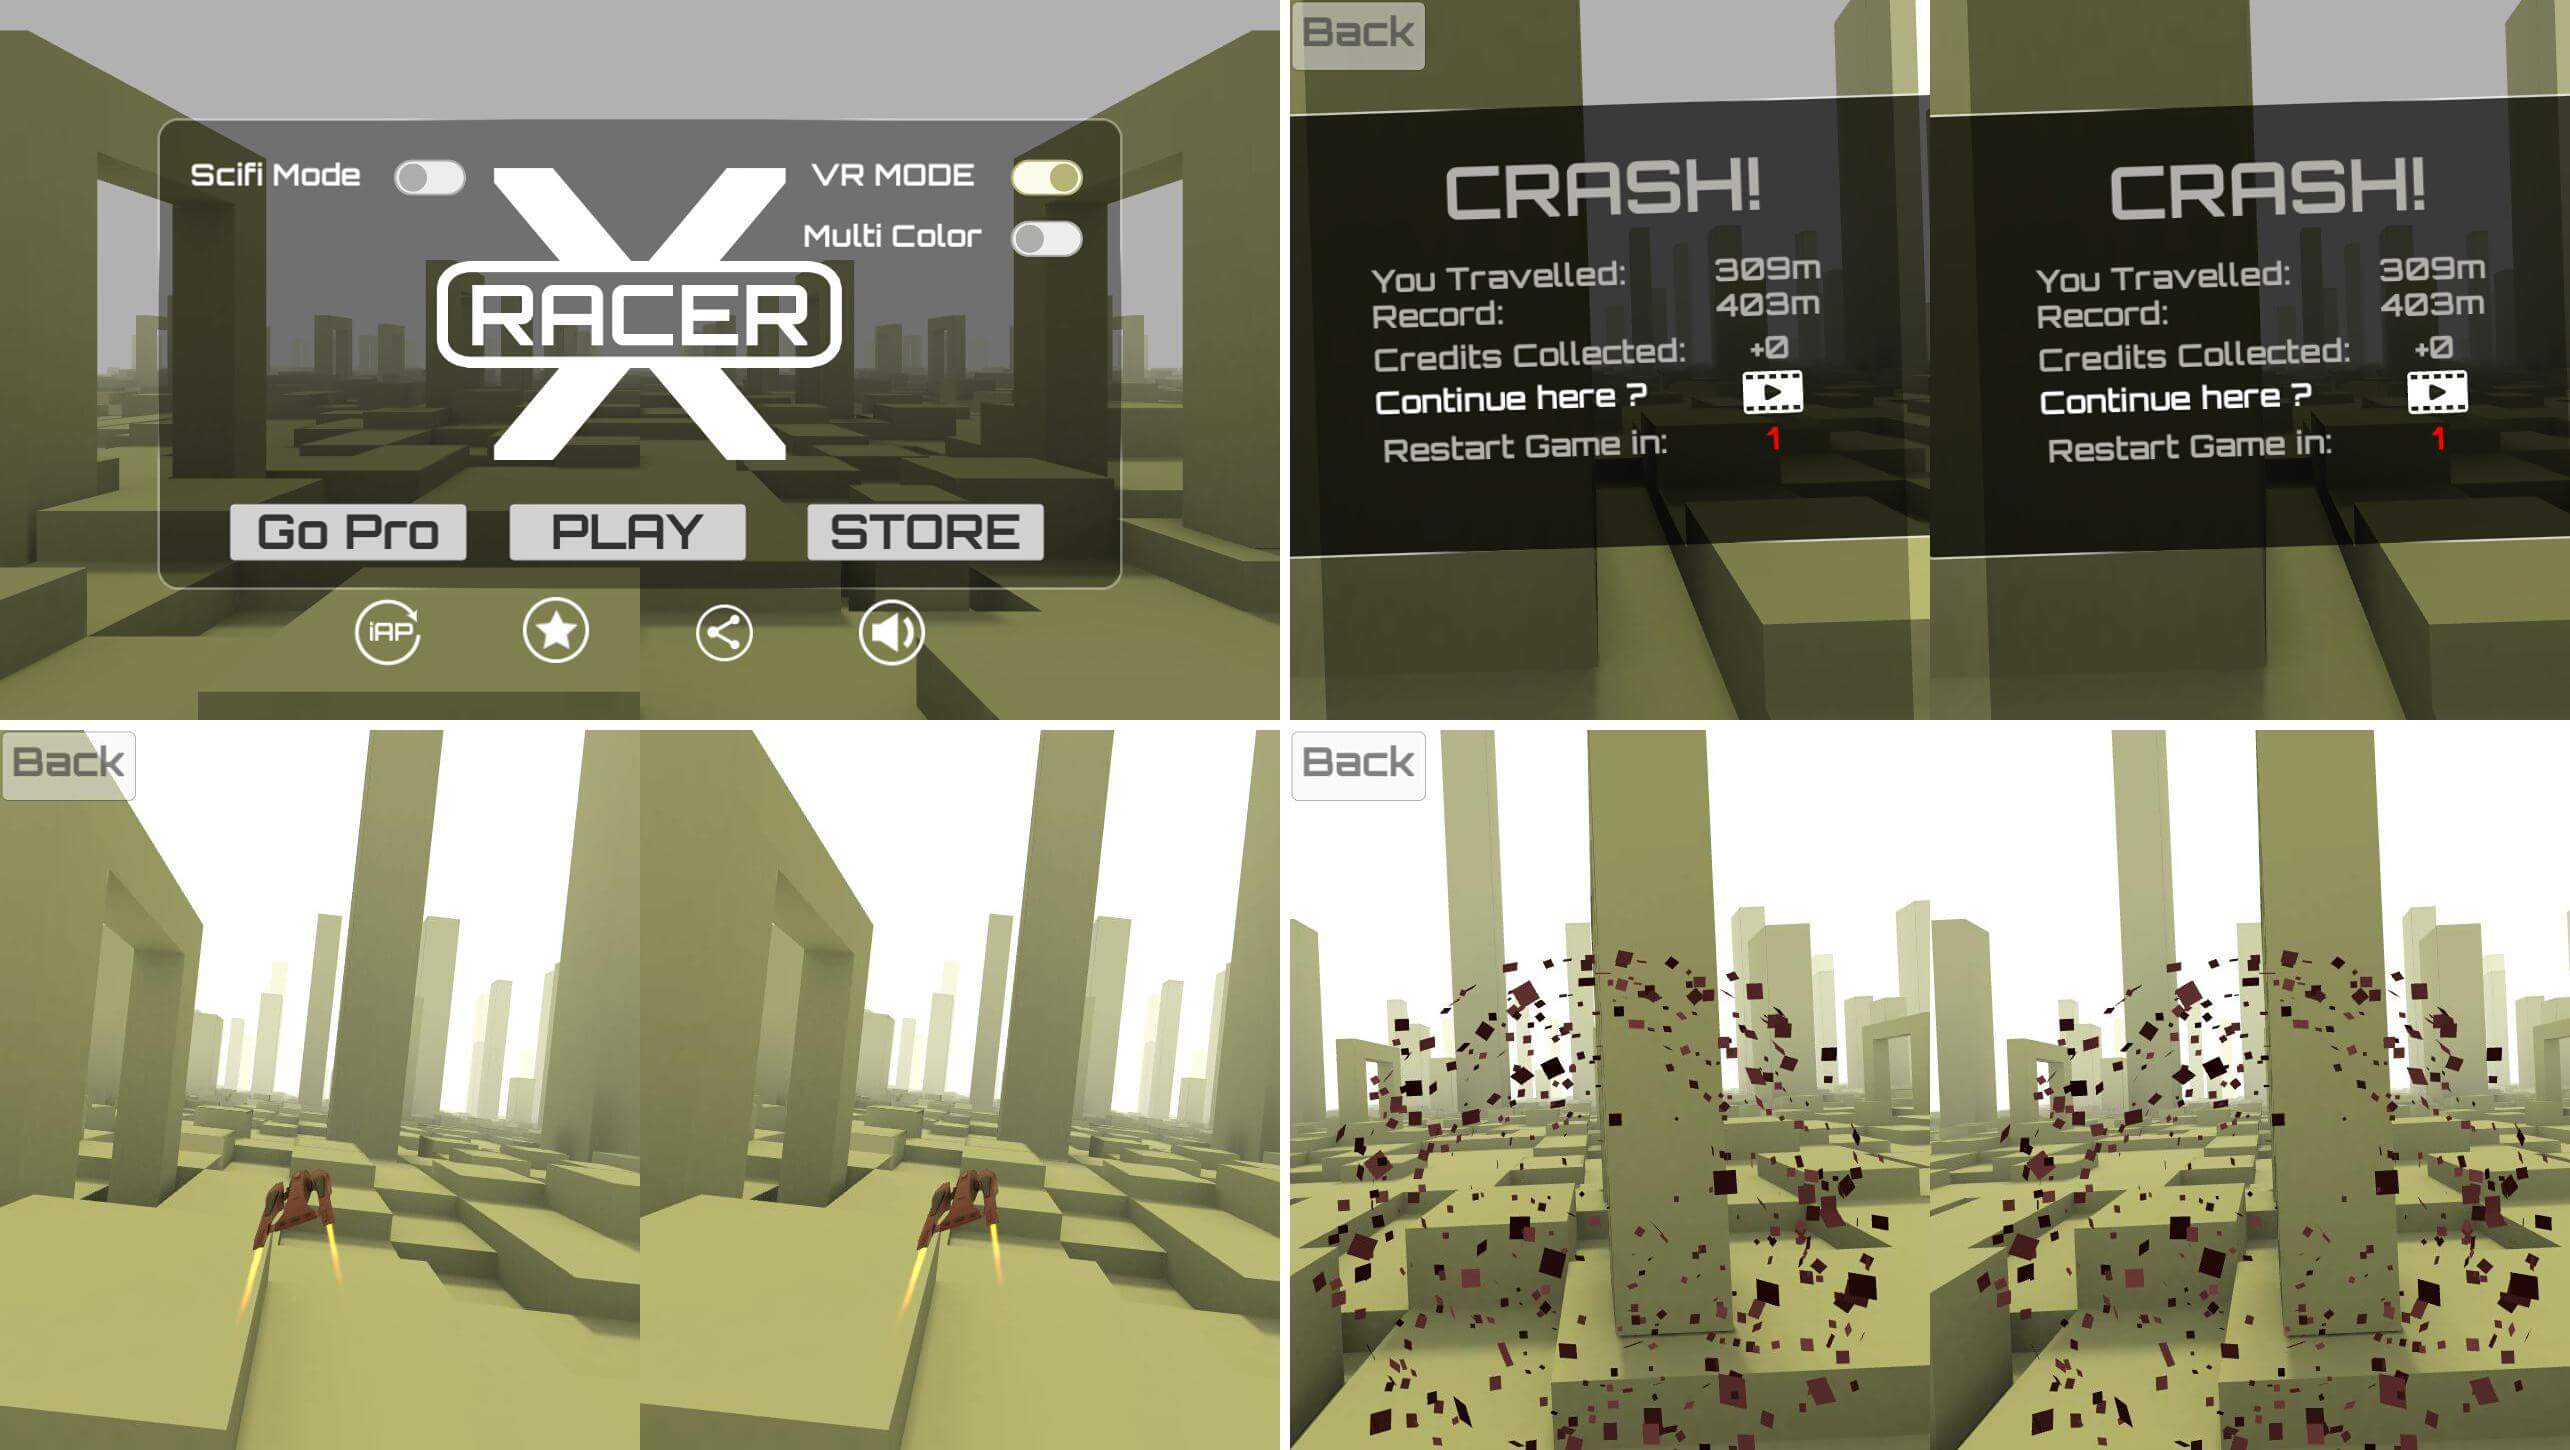
\includegraphics[width=.5\textwidth]{x-racer}
}
\caption{X-racer 游戏截图}
\label{fig:x-racer}
\end{figure}

\subsection{暴风魔镜 VR}

暴风影音是国内在全景漫游生态领域探索前沿的产品之一,最早产品发布于 2014 年,其高端产品售价可达数千元,甚至与国外高端虚拟现实设备如 Oculus 和 GearVR 等价格相齐。与其硬件设备配套的则是一款叫做“暴风魔镜 VR”的手机移动应用。

国内移动应用的发展方向一直是“大而全”,这款应用也不例外。暴风魔镜 VR 力图包括网络/本地视频、影音播放与 VR 移动应用等多种应用,形成自己的 VR 平台体系。该应用不但支持普通的移动应用界面操作模式并且同样支持全景漫游的虚拟现实体验模式。

在交互形式上与上文所列举的 Fulldive 类似,均为视线聚焦停留数秒视为确认,但缺少了语音识别输入大段文字的功能(在页面模式下支持手机输入法输入),如图\ref{fig:storm}。总体使用可满足基本的全景漫游体验,但识别速度较慢或误识别是比较严重的问题。

值得注意的一点是,暴风魔镜 VR 移动应用内场景下方有一个“归位”图标,触发后将会调整屏幕主视域至正对当前屏幕的位置,可类比于传统移动应用的“回到顶部”功能。这个功能很方便地起到了定位自身的作用,让用户不必盲目转动来寻找起始时正对着的界面。


\begin{figure}[htp]
\centering
\fbox{
  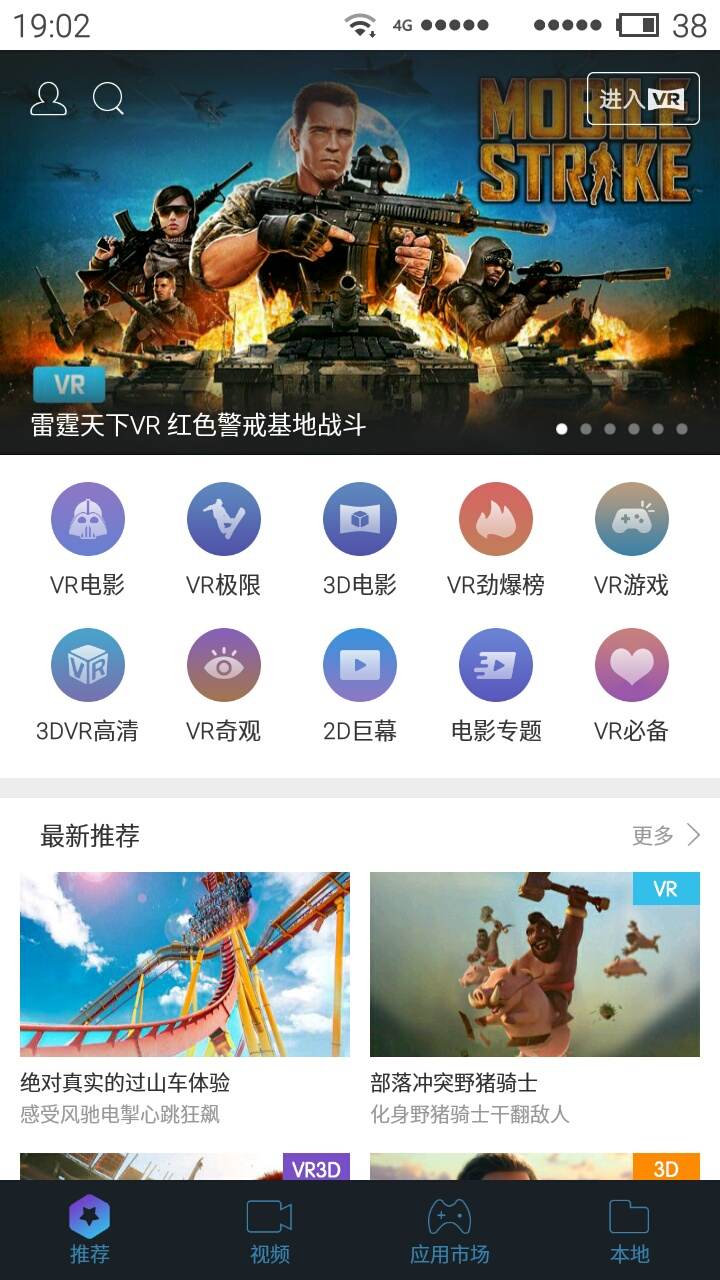
\includegraphics[width=.22\textwidth]{storm1}
}
\fbox{
  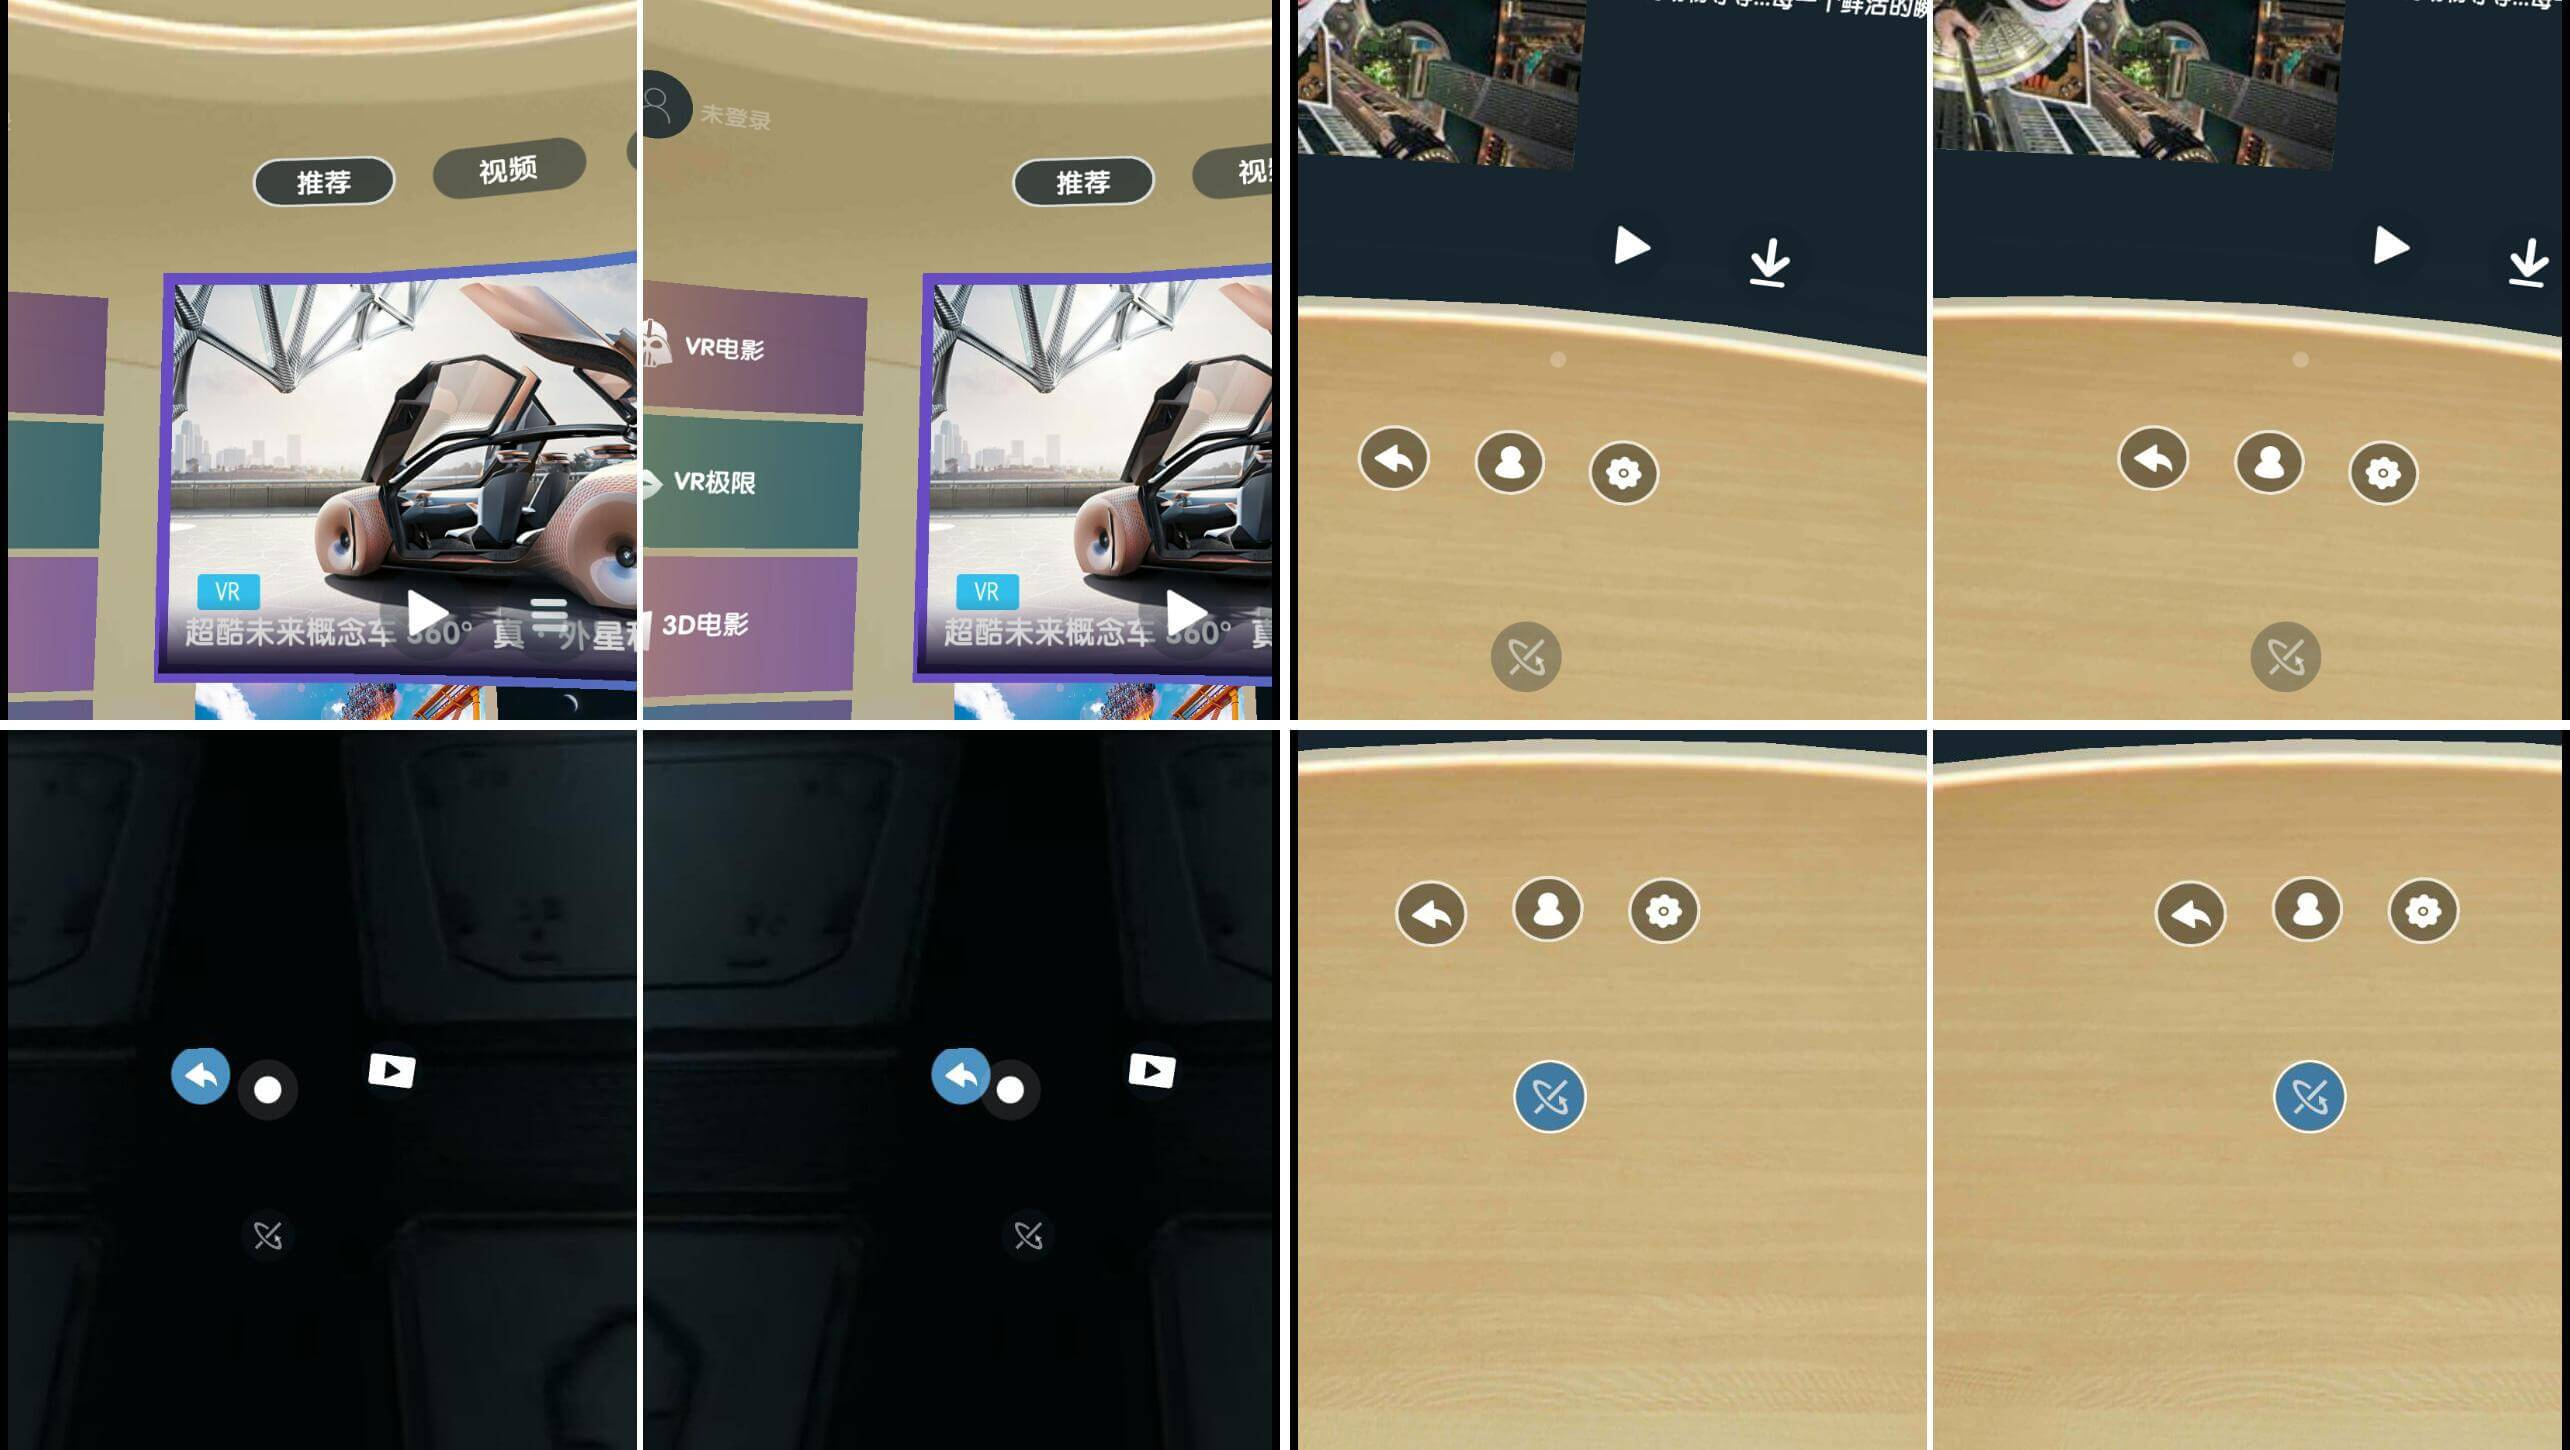
\includegraphics[width=.68\textwidth]{storm2}
}
\caption{暴风魔镜 VR 操作方式}
\label{fig:storm}
\end{figure}

\subsection{国内外移动应用总结}
国外应用较多为单一功能并凸显自身用户体验特色,而国内应用多期望建成平台式产品力图获得更大的市场份额。究其原因,国外此类开发团队小而精,立足于开发特定使用情景和目的的产品,而国内应用常常依附于配套开发的硬件设备,整体呈闭源趋势,故应用局限性较大。国外应用功能较为精简,国内应用则力图提供尽可能多的交互操作形式,但同样在交互层面难以摆脱移动设备平面屏幕所框定的范围。
